\documentclass[a4paper,12pt,twoside]{article}

\usepackage[ngerman,english]{babel}

%%% FOR DISPLAYING CODE
\usepackage[procnames]{listings}
\usepackage{xcolor}

%%% MARGINS
\usepackage{geometry}
% INFO: https://www.overleaf.com/learn/latex/Page_size_and_margins
\geometry{
	a4paper,
%	total={170mm,257mm},
	left=25mm,
	top=25mm,
	textwidth=16cm,
	textheight=23cm,
%	right=25mm,
%	bottom=40mm,$
}

%%% SPACING
%\usepackage{setspace} 
%\onehalfspacing

\usepackage{siunitx} % for writing numbers with units % e.g. \SI{6.3e8}{km}, \ang{62.59}, \num{100}'s \si{km}, \SI{53}{\degree}
\usepackage{amsmath,amssymb}
\usepackage{graphicx}
\usepackage{datetime} 
\usepackage{color}
\usepackage{float} %without it, tables position more or less random, with this an writing \begin{table}[H] the table appears right where it is defined!
\usepackage{mathptmx}
\usepackage{enumitem}

\usepackage[T1]{fontenc}
\usepackage[utf8]{inputenc}

\usepackage{pgfplots} % for plotting functions
\pgfplotsset{compat=1.16}

%%% HEADER and FOOTER
%\usepackage[automark,headsepline]{scrpage2}
%\ihead[]{\headmark}
%\chead[]{}
%\ohead[]{\pagemark}
%\ifoot[]{}
%\cfoot[\pagemark]{}
%\ofoot[]{}
%\pagestyle{scrheadings}

\usepackage{lipsum}

%% LINE SPACING
\usepackage{setspace}
\setstretch{1.5}

%%% HYPERLINKS
\usepackage{hyperref} % muss sich vor cite stuff befinden

%% SET IMAGE PATH (where images are stored)
\graphicspath{{figures/}}

%%% CITE
\usepackage{apacite}
\bibliographystyle{apacite}

%%%%%%%%%%%%%%%%%%%%%%%%%%%%%%%%%%
% DEFINE COLORS
\definecolor{red}{rgb}{0.6,0,0} 
\definecolor{blue}{rgb}{0,0,0.6}
\definecolor{green}{rgb}{0,0.8,0}
\definecolor{cyan}{rgb}{0.0,0.6,0.6}

\definecolor{mypink}{rgb}{0.753,0.000,0.890}
\definecolor{myblue}{rgb}{0.078,0.000,1.000}
\definecolor{mybluedark}{rgb}{0.004,0.024,0.525} \definecolor{mygreen}{rgb}{0.000,0.514,0.000}
\definecolor{myreddark}{rgb}{0.698,0.000,0.008}
\definecolor{mycyan}{rgb}{0.000,0.506,0.612}
\definecolor{mybrown}{rgb}{0.494,0.365,0.090}

%%% DISPLAY CODE
\usepackage{listings}
\newcommand\pythonstyle{\lstset{
    language=Python,
	tabsize=4,
	basicstyle=\normalsize\sffamily,
	numberstyle=\color{gray},
	stringstyle=\color{myreddark},
    commentstyle=\color{mygreen},
    % KEYWORDS
    % main keywords
	keywordstyle=\normalsize\color{myblue},%\bfseries,
    % add keywords (main blue)
    emph={False,None,True,self,TODO},
    emphstyle={\color{myblue}},
    % pink emph
    emph={[2]assert,break,continue,del,elif ,else,except,finally,for,from,global,if,import,in,pass,raise,return,try,while,with,yield},
    emphstyle={[2]\color{mypink}},%\bfseries,
    %dark blue emph
    emph={[3]execfile,reduce,xrange},
    emphstyle={[3]\color{mybluedark}},
    % brown emph
    emph={[4]exec,print,isinstance,zip,enumerate,reversed,len,repr},
    emphstyle={[4]\color{mybrown}},
    % cyan emph
    emph={[5]object,type,list,set,dict,tuple,str,super},
    emphstyle={[5]\color{mycyan}},
    % errors (also cyan emph)
    emph={[6]Exception,NameError,IndexError,SyntaxError,TypeError,ValueError,OverflowError,ZeroDivisionError},
    emphstyle={[6]\color{mycyan}},
    % errors (also cyan emph)
    emph={[7]copy,deepcopy,append,real,imag},
    emphstyle={[7]\color{black}},
    % 
    showstringspaces=false,
	breaklines=true,
	numbers=left,
    frame=tb,
	xleftmargin=15pt
}}

\newcommand\javascriptstyle{\lstset{
	basicstyle=\small\sffamily,
    keywordstyle=\color{blue}\bfseries,
    commentstyle=\color{purple}\ttfamily,
    stringstyle=\color{red}\ttfamily,
	numberstyle=\color{gray},
    keywords={typeof, new, true, false, catch, function, return, null, catch, switch, var, if, in, while, do, else, case, break},
    ndkeywords={class, export, boolean, throw, implements, import, this},
    ndkeywordstyle=\color{darkgray}\bfseries,
    identifierstyle=\color{black},
    comment=[l]{//},
    morecomment=[s]{/*}{*/},
    morestring=[b]',
    morestring=[b]",
    showstringspaces=false,
	breaklines=true,
	numbers=left,
    frame=tb,
	xleftmargin=15pt,
    sensitive=false,
}}

\newcommand\csharpstyle{\lstset{
	language=csh,
	tabsize=4,
	basicstyle=\small\sffamily,
	numberstyle=\color{gray},
	stringstyle=\color{myreddark},
    commentstyle=\color{mygreen},
	morecomment=[l]{//}, %use comment-line-style!
	morecomment=[s]{/*}{*/}, %for multiline comments
    % KEYWORDS
	keywordstyle=\normalsize\color{myblue},%\bfseries,
	morekeywords={ abstract, event, new, struct,
		as, explicit, null, switch,
		base, extern, object, this,
		bool, false, operator, throw,
		break, finally, out, true,
		byte, fixed, override, try,
		case, float, params, typeof,
		catch, for, private, uint,
		char, foreach, protected, ulong,
		checked, goto, public, unchecked,
		class, if, readonly, unsafe,
		const, implicit, ref, ushort,
		continue, in, return, using,
		decimal, int, sbyte, virtual,
		default, interface, sealed, volatile,
		delegate, internal, short, void,
		do, is, sizeof, while,
		double, lock, stackalloc,
		else, long, static,
		enum, namespace, string},
	% 
    showstringspaces=false,
	breaklines=true,
	numbers=left,
    frame=tb,
	xleftmargin=15pt	
}}

% Python environment
\lstnewenvironment{python}[1][]
{
	\pythonstyle
	\lstset{#1}
}
{}
\lstnewenvironment{javascript}[1][]
{
	\javascriptstyle
	\lstset{#1}
}
{}
\lstnewenvironment{csharp}[1][]
{
	\csharpstyle
	\lstset{#1}
}
{}

% CODE FOR EXTERNAL FILES
\newcommand\pythonexternal[2][]{{
		\pythonstyle
		\lstinputlisting[#1]{#2}}}

% CODE FOR INLINE
\newcommand\pythoninline[1]{{\pythonstyle\lstinline!#1!}}
\newcommand\csharpinline[1]{{\csharpstyle\lstinline!#1!}}
\newcommand\javascriptinline[1]{{\javascriptstyle\lstinline!#1!}}

%% DEFINE CUSTOM COMMANDS AND SHORTCUTS

% some commands
\def\ba#1\ea{\begin{align}#1\end{align}}
\def\bas#1\eas{\begin{align*}#1\end{align*}}
\def\bmat#1\emat{\begin{pmatrix}#1\end{pmatrix}}
\newcommand{\ve}[1]{\vec{#1}}
\newcommand{\veTwo}[2]{\begin{pmatrix}#1\\#2\end{pmatrix}}
\newcommand{\veThree}[3]{\begin{pmatrix}#1\\#2\\#3\end{pmatrix}}
\newcommand{\veFour}[4]{\begin{pmatrix}#1\\#2\\#3\\#4\end{pmatrix}}
\newcommand{\ora}[1]{\overrightarrow{#1}}
\newcommand{\ola}[1]{\overleftarrow{#1}}
\newcommand{\s}[1]{\sqrt{#1}}

\def \bit{\begin{itemize}\setlength\itemsep{0em}} %\vspace{-5mm}
	\def \eit{\end{itemize}}

\def \ben{\begin{enumerate}\setlength\itemsep{0em}} %\vspace{-5mm}
	\def \een{\end{enumerate}}

\def \N{\mathbb{N}}
\def \Z{\mathbb{Z}}
\def \Q{\mathbb{Q}}
\def \R{\mathbb{R}}
\def \C{\mathbb{C}}

\def \ra{\rightarrow}
\def \longra{\longrightarrow}
\def \Ra{\Rightarrow}
\def \Longra{\Longrightarrow}
\def \la{\leftarrow}
\def \longla{\longleftarrow}
\def \La{\Leftarrow}
\def \Longla{\Longleftarrow}

\def \lra{\leftrightarrow}
\def \longlra{\longleftrightarrow}
\def \Lra{\Leftrightarrow}
\def \Longlra{\Longleftrightarrow}

\def \l{\left}
\def \r{\right}

\def \a{\alpha}
\def \b{\beta}
\def \g{\gamma}

\def \c{\cdot}

\def \el{\in}
\def \notel{\notin}

\newcommand{\f}{\frac}

\def \q{\quad}
\newcommand{\p}{\phantom}

\def\bs#1\es{\begin{split}#1\end{split}}


\def \L{\mathbb{L}}




\begin{document}

%%%%%%%%%%%%%%%%%%%%%%%%%%%%%%%%%%%%%%%%%%%%%%%%%%%%%%%
%%%%%%%%%%%%%%%%%%%%%%%%%%%%%%%%%%%%%%%%%%%%%%%%%%%%%%%
%%%%%%%%%%%%%%%%%%%%%%%%%%%%%%%%%%%%%%%%%%%%%%%%%%%%%%%

%%% AB HIER ARBEITEN, WEITER OBEN NICHTS VERAENDERN
%%% Ausnahme: Einbinden weitere Pakete

\selectlanguage{ngerman} %% HIER SPRACHE EINSTELLEN! english, ngerman

\begin{titlepage}
	\clearpage\thispagestyle{empty}	
	\setstretch{1}
	
	\begin{minipage}[t]{\textwidth}
		\begin{minipage}[t]{0.5\textwidth}
			Zeynep Zülal Keskin\\
			Mattfeldstrasse 6\\
			9532 Rickenbach b. Wil\\
			077 277 43 77\\
			zekeskin@ksr.ch
		\end{minipage}
		\begin{minipage}[t]{0.5\textwidth}
			\begin{flushright}
				Kantonsschule Romanshorn\\
				Klasse 4Ma\\
				Maturaarbeit
			\end{flushright}
		\end{minipage}
	\end{minipage}
	
	\vspace{4cm}
	{
		\centering
		\Huge\bfseries N-Körper Problem\par
		\vspace{1cm}
		\includegraphics[width=0.15\textwidth]{example-image-1x1}\par
	}
	
	\vspace{9cm}	
	\noindent
    Fach: Physik, Mathematik, Informatik \noindent\\
	Betreuungsperson: Dr. Andreas Schärer\\
	Abgabetermin: 6. Januar 2025
	
\end{titlepage}

%%%%%%%%%%%%%%%%%%%%%%%%%%%%%%%%%%%%%%%%%%%%%%%%%%%%%%%
%%%%%%%%%%%%%%%%%%%%%%%%%%%%%%%%%%%%%%%%%%%%%%%%%%%%%%%
%%%%%%%%%%%%%%%%%%%%%%%%%%%%%%%%%%%%%%%%%%%%%%%%%%%%%%%

% \null\thispagestyle{empty}\clearpage

%%% ABSTRACT

\pagenumbering{roman}

\section*{Abstract}

Das N-Körper-Problem ist ein fundamentales Problem der Himmelsmechanik, das die Bewegung von N Massenpunkten unter gegenseitiger gravitativer Anziehung beschreibt. Diese Arbeit untersucht zwei verschiedene Simulationsmethoden für das N-Körper-Problem: die direkte Methode und den Barnes-Hut-Algorithmus. Ziel ist es, die Genauigkeit und Effizienz dieser Methoden zu analysieren und zu vergleichen.
%%%%%%%%%%%%%%%%%%%%%%%%%%%%%%%%%%%%%%%%%%%%%%%%%%%%%%%
%%%%%%%%%%%%%%%%%%%%%%%%%%%%%%%%%%%%%%%%%%%%%%%%%%%%%%%
%%%%%%%%%%%%%%%%%%%%%%%%%%%%%%%%%%%%%%%%%%%%%%%%%%%%%%%

%%% TABLE OF CONTENTS

%\null\thispagestyle{empty}\clearpage
\newpage
%\setcounter{page}{1}
\tableofcontents

\parindent=0pt
\parskip=6pt

\newpage

\pagenumbering{arabic}

%%%%%%%%%%%%%%%%%%%%%%%%%%%%%%%%%%%%%%%%%%%%%%%%%%%%%%%
%%%%%%%%%%%%%%%%%%%%%%%%%%%%%%%%%%%%%%%%%%%%%%%%%%%%%%%
%%%%%%%%%%%%%%%%%%%%%%%%%%%%%%%%%%%%%%%%%%%%%%%%%%%%%%%

\section{Einleitung}
Diese Arbeit befasst sich mit einem der grundlegendsten und komplexesten Probleme der Himmelsmechanik und -dynamik: dem N-Körper-Problem in der Physik. Dieses Problem ist nicht nur von theoretischem Interesse, sondern findet auch praktische Anwendungen in der Astronomie, Raumfahrt und vielen anderen Bereichen der Physik. Die zentrale Forschungsfrage dieser Arbeit lautet: Welche mathematischen und physikalischen Methoden können verwendet werden, um die Bewegung von N-Körpern zu beschreiben und zu verstehen? 
Das Ziel dieser Arbeit ist es, die Bewegung von N-Körpern zu definieren und umfassend zu analysieren. Dabei soll der physikalische Hintergrund dieses Problems beleuchtet und seine historische Entwicklung nachgezeichnet werden. Ein besonderer Schwerpunkt liegt auf der Darstellung und Untersuchung der verschiedenen mathematischen und physikalischen Methoden, die im Laufe der Zeit entwickelt wurden, um die Dynamik von N-Körpern zu erklären.
Darüber hinaus werden zwei detaillierte Simulationen entwickelt, um die theoretischen Konzepte praktisch zu veranschaulichen. Diese Simulationen dienen nicht nur der Erklärung des Problems, sondern auch dem Vergleich verschiedener Lösungsansätze. Durch diese Herangehensweise soll ein tieferes Verständnis für die Komplexität des N-Körper-Problems und die Herausforderungen bei seiner Lösung vermittelt werden.
Ein weiterer Aspekt dieser Arbeit ist die Untersuchung der praktischen Relevanz des N-Körper-Problems. Dabei wird aufgezeigt, wie die theoretischen Erkenntnisse in der Astronomie zur Berechnung von Planetenbahnen, in der Raumfahrt zur Planung von Satellitenmissionen und in anderen Bereichen der Physik zur Modellierung komplexer Systeme angewendet werden können.
Zusammenfassend strebt diese Arbeit an, einen umfassenden Überblick über das N-Körper-Problem zu geben, seine Bedeutung in der modernen Physik aufzuzeigen und durch die Entwicklung und den Vergleich von Simulationen einen Beitrag zur Lösung dieses faszinierenden und herausfordernden Problems zu leisten.

\newpage
\section{Theoretische Grundlagen}

\subsection{Problembeschreibung und historische Entwicklung}
Das N-Körper-Problem beschäftigt sich mit der dynamischen Analyse von N Massepunkten, die durch ihre gegenseitige gravitative Anziehung beeinflusst werden. Während das Zwei-Körper-Problem durch Newtons Gesetz der universellen Gravitation und die Keplerschen Gesetze exakt gelöst werden kann, wird das N-Körper-Problem für N Körper wesentlich komplexer und zeigt in der Regel chaotisches Verhalten. Die historische Entwicklung dieses Problems begann im 17. Jahrhundert mit den grundlegenden Arbeiten von Johannes Kepler und Isaac Newton, die die Basis für die Himmelsmechanik schufen. Im 18. und 19. Jahrhundert erweiterten Joseph-Louis Lagrange und Pierre-Simon Laplace das Verständnis durch die Einführung der Lagrangeschen Gleichungen und durch die Analyse spezieller Lösungen wie der Lagrange-Punkte, die besondere Gleichgewichtslagen in einem gravitativen System beschreiben. Henri Poincaré entdeckte Ende des 19. Jahrhunderts die chaotische Natur des Systems, was den Beginn der modernen Chaosforschung einleitete. Im 20. und 21. Jahrhundert ermöglichten Fortschritte in der Computertechnologie und numerischen Methoden präzise Simulationen und Analysen komplexer N-Körper-Systeme, die wichtige Einblicke in die Dynamik von Galaxien und die Planung von Raumfahrtmissionen bieten.

\subsection{Gravitationskraft}
Die Gravitationskraft $\vec{F}_{12}$ zwischen zwei punktförmigen Massen $m_1$ und $m_2$ liegt auf der Verbindungslinie der beiden Massen. Der Betrag $F$ der Gravitationskraft ist proportional zu den Massen $m_1$ und $m_2$ sowie umgekehrt proportional zum Quadrat des Abstands $r$ (die relative Position ist die Position eines Körpers relativ zu einem anderen: \(\vec{r} = \vec{r}_2 - \vec{r}_1\)) der Massen. Er berechnet sich durch:
\begin{align*}
	F = G \frac{m_1 m_2}{r^2}
\end{align*}
mit der Gravitationskonstante $G = \SI{6.674e-11}{\frac{m^3}{kg\,s^2}}$.

\subsection{Die Keplerschen Gesetze}
Die Keplerschen Gesetze beschreiben die Bewegung von Planeten um die Sonne und sind grundlegende Prinzipien der Himmelsmechanik. Johannes Kepler formulierte sie im frühen 17. Jahrhundert auf Basis der Beobachtungen von Tycho Brahe. Diese Gesetze markierten einen Wendepunkt von der klassischen, kreisförmigen Vorstellung der Planetenbewegung zu einem elliptischen Modell. Im Folgenden werde ich die drei Keplerschen Gesetze erläutern.
\subsubsection{1. Keplersches Gesetz: Das Gesetz der Ellipsen}
Das erste Keplersche Gesetz besagt:
\begin{quote}
    Die Bahnen der Planeten um die Sonne sind Ellipsen, wobei sich die Sonne in einem der beiden Brennpunkte befindet.
\end{quote}
Mathematisch lässt sich eine Ellipse durch die Gleichung
\begin{align*}
	\frac{x^2}{a^2} + \frac{y^2}{b^2} = 1
\end{align*}

beschreiben, wobei \(a\) die große Halbachse und \(b\) die kleine Halbachse der Ellipse ist. Der Planet bewegt sich auf einer solchen Ellipsenbahn, wobei sich die Sonne nicht im Zentrum der Ellipse befindet, sondern in einem der beiden Brennpunkte. Dies war ein entscheidender Unterschied zur zuvor angenommenen Kreisbahn der Planeten.
\subsubsection{2. Keplersches Gesetz: Das Gesetz der Flächen}
Das zweite Keplersche Gesetz lautet:

\begin{quote}
    Der Fahrstrahl (die Verbindungslinie) zwischen einem Planeten und der Sonne überstreicht in gleichen Zeitspannen gleiche Flächen.
\end{quote}
Dies bedeutet, dass sich ein Planet auf seiner elliptischen Bahn unterschiedlich schnell bewegt: Er ist schneller, wenn er sich näher an der Sonne befindet (Perihel) und langsamer, wenn er weiter entfernt ist (Aphel). Dies lässt sich mathematisch durch die Erhaltung des Drehimpulses ausdrücken, da der Winkelgeschwindigkeitsvektor und der Abstand zur Sonne in Beziehung stehen. Formal lässt sich dies auch durch die Flächengeschwindigkeit beschreiben:
\begin{align*}
	\frac{dA}{dt} = \text{konstant},
\end{align*}

wobei \(A\) die Fläche und \(t\) die Zeit ist. Diese Konstanz der Flächengeschwindigkeit ist ein Hinweis auf das Prinzip der Erhaltung des Drehimpulses.

\subsubsection{3. Keplersches Gesetz: Das Harmoniegesetz}
Das dritte Keplersche Gesetz beschreibt die Beziehung zwischen der Umlaufzeit eines Planeten und seiner Entfernung von der Sonne:
\begin{quote}
    Die Quadrate der Umlaufzeiten zweier Planeten verhalten sich wie die Kuben der großen Halbachsen ihrer Bahnen.
\end{quote}
Mathematisch wird dies durch die Gleichung
\begin{align*}
	\frac{T_1^2}{T_2^2} = \frac{a_1^3}{a_2^3}
\end{align*}

ausgedrückt, wobei \(T_1\) und \(T_2\) die Umlaufzeiten der beiden Planeten und \(a_1\) und \(a_2\) die großen Halbachsen ihrer Bahnen sind. Dies zeigt, dass Planeten, die weiter von der Sonne entfernt sind, eine längere Umlaufzeit haben als solche, die sich näher an der Sonne befinden.

\subsection{Zwei-Körper-Problem}
Das Zweikörperproblem besteht darin, die Bahnen von zwei gravitativ wechselwirkenden Körpern mit bekannten Massen und Anfangsgeschwindigkeiten zu bestimmen. 
Die Körper bewegen sich im dreidimensionalen Raum und werden von keinen anderen Kräften außer der Gravitationskraft beeinflusst. Die erste Lösung des Zweikörperproblems wurde 1687 von Isaac Newton in seinem bahnbrechenden Werk Principia veröffentlicht. 
Im 17. Jahrhundert zeigte Johannes Kepler, dass die Planetenbahnen um die Sonne elliptisch sind. Dies war für seine Zeitgenossen erstaunlich, da sie den Kreis als die göttliche Form ansahen, die die Himmelskörper regierte. 
Kepler steckte viel Mühe in seine Berechnungen und nutzte dabei die Beobachtungsdaten von Tycho Brahe. Trotz seiner Entdeckungen konnte er jedoch nie erklären, warum sich die Planeten so bewegen, wie sie es tun. Einige glaubten, dass sie von Engeln vorangetrieben wurden. 
Eine andere populäre Idee, die von René Descartes vorgeschlagen wurde, erklärte die Bewegung durch Wirbel von Partikeln, die den gesamten Raum füllten (Densmore [2003]). 
Newton revolutionierte die Welt, indem er ihr das universelle Gravitationsgesetz gab ein Gesetz, das die Bewegung im konstanten Gravitationsfeld sowohl auf der Erde als auch die Bewegungen der Planeten erklären konnte. 
Manche verspotteten diese Theorie und bezeichneten eine unsichtbare Kraft als übernatürlich und okkult. Einige hundert Jahre später, als die Newtonsche Mechanik zu einem der Hauptpfeiler der modernen Physik wurde, finden wir Theorien über Engel oder Wirbel im Weltraum amüsant. Angesichts unseres heutigen Wissens ist es schwer, sich die Herausforderungen vorzustellen, denen sich Newton als Wissenschaftler stellen musste, und aus welcher Denkweise heraus er wissenschaftliche 
Normen durchbrechen konnte. Ein weiteres Hindernis, dem Wissenschaftler im 17. Jahrhundert begegneten, war der Mangel an Daten, um neue Theorien zu überprüfen. Als Newton während eines langen Aufenthalts bei seiner Mutter in Woolsthorpe die Idee der Gravitation entwickelte, wollte er sie testen, indem er die Umlaufbahn des Mondes berechnete.


\subsubsection{Die Mathematische Beschreibung}

Da nur die zwei Körper (Massen \( m_1, m_2 \), Orte \( \vec{x_1}, \vec{x_2} \)) aufeinander einwirken, heißen die Bewegungsgleichungen:

\begin{align*}
	m_1 \ddot{\vec{x}}_1 &= \vec{F}_{1,2} \\
	m_2 \ddot{\vec{x}}_2 &= \vec{F}_{2,1}
\end{align*}

Dabei können die Kräfte \( \vec{F}_{1,2}, \vec{F}_{2,1} \) nach dem Relativitätsprinzip nur von der relativen Position der Körper zueinander abhängen. Der Vektor \( \vec{r} := \vec{x_1} - \vec{x_2} \) beschreibt die Lage des zweiten Körpers relativ zum ersten, der Vektor \( \vec{R} \) ist der Ortsvektor des Schwerpunkts oder Baryzentrums des Systems. Zudem sind die beiden Kräfte nach dem 3. Newtonschen Axiom entgegengesetzt gleich:

\begin{align*}
\vec{F}_{1,2} = -\vec{F}_{2,1} = \vec{F}(\vec{r})
\end{align*}

\subsubsection{Übergang zum äquivalenten Einkörperproblem}
Mathematische Modellierung der Lage zweier Körper im Raum und sind vom Koordinatenursprung 
ausgehende Positionsvektoren. Man rechnet nun in Relativ- und Schwerpunktkoordinaten (siehe Abbildung 1).
\begin{figure}[H]
	\centering
	\includegraphics[width=0.4\textwidth]{Zwei-Körper.png}
	\caption[Eintrag in Abbildungsverzeichnis von Grumpy Cat]{Mathematische Modellierung der Lage zweier Körper im Raum, x1 und x2 sind vom Koordinatenursprung ausgehende Positionsvektoren.}
	\label{Zwei-Körper .}
\end{figure}

\begin{align*}
	\vec{r} &= \vec{x_1} - \vec{x_2} \\
	\vec{R} &= \frac{m_1 \vec{x_1} + m_2 \vec{x_2}}{M} \quad (M = m_1 + m_2 \text{ ist die Gesamtmasse.})
\end{align*}

Durch Addition geeigneter Vielfacher der beiden obigen Bewegungsgleichungen erhält man nun zwei entkoppelte Bewegungsgleichungen:

\begin{align*}
	\ddot{\vec{R}} &= 0 \\
	\vec{r} &= \left( \frac{1}{m_1} + \frac{1}{m_2} \right) \vec{F}_{1,2}
\end{align*}


Die erste Gleichung besagt, dass der Massenschwerpunkt eine geradlinig gleichförmige Bewegung beschreibt, wie es auch aus dem allgemeinen Schwerpunktsatz zu folgen ist. Die zweite Gleichung wird umformuliert zu:

\begin{align*}
\mu \ddot{\vec{r}} = \vec{F}(\vec{r}),
\end{align*}

wobei,

\begin{align*}
\mu = \left( \frac{1}{m_1} + \frac{1}{m_2} \right)^{-1} = \frac{m_1 m_2}{M}
\end{align*}
als die \textit{reduzierte Masse} des Zweikörperproblems bezeichnet wird. $\mu$ ist stets kleiner als die kleinere der beiden Massen, und nähert sich ihr an, wenn die größere Masse gegen unendlich strebt. Diese Bewegungsgleichung besagt, dass die Relativkoordinate $\vec{r}(t)$ sich so verhält, als ob ein Körper der Masse $\mu$ sich in einem ortsfesten Kraftfeld $\vec{F}(\vec{r})$ bewegt. Dies ist das äquivalente Einkörperproblem. Für alle Fälle, in denen die Stärke der Kraft von einer Potenz des Abstandes $r$ abhängt, ist es zuerst von Newton gelöst worden.

\subsubsection{Gemeinsame Bewegung}
Nachdem das Einkörperproblem durch die Bahnkurve $\vec{r}(t)$
gelöst ist und die Bewegung des Schwerpunktes $\vec{R}(t)$
ebenfalls bekannt ist, kann man wieder in die ursprünglichen Koordinaten umrechnen:

\begin{align*}
	\vec{x_1}(t) &= \vec{R}(t) + \frac{m_2}{M} \vec{r}(t) \\
	\vec{x_2}(t) &= \vec{R}(t) - \frac{m_1}{M} \vec{r}(t)
\end{align*}
Im Schwerpunktsystem betrachtet (mathematisch, indem man eine Koordinatentransformation, genauer eine Verschiebung, um \( \mathbf{R} \) anwendet), bewegen sich also beide Körper um den Schwerpunkt, der stets auf ihrer Verbindungsline liegt, und beschreiben zwei zur Kurve \( \mathbf{r}(t) \) ähnliche Kurven, deren Größenverhältnis durch das resiproke Massenverhältnis bestimmt ist. Durch zweimaliges Differenzieren von \( \mathbf{x_1}(t) \) und Einsetzen von

\begin{align*}
	\vec{r} = \frac{M}{m_2} \vec{x_1}
\end{align*}

sieht man, dass für den ersten Körper die Bewegungsgleichung:

\begin{align*}
	m_1 \ddot{\vec{x}}_1 = \vec{F}_{\text{eff}}(\vec{x_1})
\end{align*}

erfüllt ist, als ob der Körper sich in einem effektiven Kraftfeld:

\begin{align*}
	\vec{F}_{\text{eff}}(\vec{x_1}) = \vec{F} \left( \frac{M}{m_2} \vec{x_1} \right)
\end{align*}

bewegen würde, dessen Zentrum ortsfest am Schwerpunkt bleibt und dessen Stärke mit dem wirklichen Kraftfeld in einer durch das Massenverhältnis bestimmten größeren Entfernung übereinstimmt - genauso für den anderen Körper.
Wenn sich der Schwerpunkt selbst geradlinig und gleichförmig bewegt, und weitere geeignete Startbedingungen erfüllt sind, dann beschreiben die Bahnen der beiden Körper eine Art „Schlangenkurve“ um die Bahn des Schwerpunktes. In der Astronomie erlaubt diese sogenannte Taumelbewegung eine indirekte Beobachtung unsichtbarer Begleiter von Sternen wie z. B. Exoplaneten.

\subsubsection{Drehimpulserhaltung}
Die Kraft \( \vec{F}_{1,2} = -\vec{F}_{2,1} = \vec{F}(\vec{r}) \) liegt parallel zur Verbindungsline \( \vec{r} \) (entsprechend der Problemdefinition), deshalb ist sie eine Zentralkraft und übt kein Drehmoment auf den umlaufenden Körper aus, denn dieses ist durch das Vektorprodukt von Radiusvektor und Kraft gegeben:

\begin{align*}
	\vec{r} \times \vec{F} = 0
\end{align*}

Daher ist der Drehimpuls \( \vec{L} = \vec{r} \times \vec{p} \) nach Betrag und Richtung zeitlich konstant. Er ist ein Integral der Bewegung. Somit erfolgt die Bewegung in einer festen Ebene, denn die Vektoren \( \vec{r} \) und \( \vec{p} = \mu \vec{r} \) liegen stets in der Ebene senkrecht zu \( \vec{L} \).
Aus der Konstanz des Drehimpulses folgt auch das 2. Keplersche Gesetz oder der Flächensatz, der also für jedes Zentralkraftfeld gilt.
In ebenen Polarkoordinaten zerfällt die vektorielle Bewegungsgleichung des Einkörperproblems in zwei gekoppelte gewöhnliche Differentialgleichungen:

\begin{align*}
	\dot{r} - r \dot{\varphi}^2 = - \frac{1}{\mu} F(r) \\
	\frac{d}{dt} \left( \mu r^2 \dot{\varphi} \right) = 0
\end{align*}
Die zweite dieser Gleichungen zeigt noch einmal die Erhaltung des Drehimpulses \( L \), denn

\begin{align*}
	L = \mu r^2 \dot{\varphi}
\end{align*}


\subsubsection{Energieerhaltung}
Für das Keplerproblem im engeren Sinn ist die Kraft durch die Gravitation gegeben:

\begin{align*}
	F(r) = - \frac{G m_1 m_2}{r^2}
\end{align*}
Verwendet man die Definition des Drehimpulses in Polarkoordinaten, um aus der anderen Differentialgleichung die Winkelgeschwindigkeit \( \dot{\varphi} \) zu eliminieren, erhält man ein Gesetz für den Abstand \( r \), die Radialgleichung

\begin{align*}
	\mu \ddot{r} = \frac{L^2}{\mu r^3} - \frac{G M}{r^2}
\end{align*}
Dies kann nach Multiplikation mit \( \dot{r} \) und \( \mu \) in der Form
\begin{align*}
	\frac{d}{dt} \left( \frac{\mu}{2} \dot{r}^2 + \frac{L^2}{2 \mu r^2} - \frac{GM \mu}{r} \right) = 0
\end{align*}
geschrieben werden. Die drei Summanden in dieser Gleichung entsprechen der Reihenfolge nach dem Radialanteil der kinetischen Energie, dem Winkelanteil der kinetischen Energie, der als Zentrifugalpotential wie eine potentielle Energie die Radialbewegung beeinflusst, sowie der potentiellen Energie des Körpers im äußeren Zentralpotential. Gemeinsam ergeben sie seine Gesamtenergie:
\begin{align*}
	E = \frac{\mu}{2} \dot{r}^2 + \frac{L^2}{2 \mu r^2} - \frac{GM \mu}{r}
\end{align*}
die laut obiger Gleichung zeitlich konstant und somit ebenfalls ein Integral der Bewegung ist. Die Gesamtenergie muss natürlich schon allein deshalb erhalten sein, weil es sich bei einem Gravitationsfeld um ein konservatives Feld handelt. Genau auch den Artikel Spezifische Bahnenenergie, der sich näher damit befasst.


\subsubsection{Bahnkurve-Kegelschnittform}

Gibt man die Werte für die beiden Integrale der Bewegung \( E \) und \( L \) vor, so lässt sich die Bewegungsgleichung lösen, indem man zunächst die radiale Bewegung \( r(t) \) aus der Form des Energieintegrals (letzte Gleichung im obigen Abschnitt) und sodann die Winkelbewegung \( \varphi(t) \) aus dem Drehimpulsintegral \( L = \mu r^2 \dot{\varphi} \) berechnet. 
Allerdings führt dieser Weg auf Gleichungen, die man als unanschaulich erkennen kann, da man ihnen die Form der Bahn nicht direkt ansehen kann.
Daher ist es üblich, entweder die Radialgleichung oder das Energieintegral zunächst in eine Differentialgleichung nach dem Winkel \( \varphi \) umzuwandeln. Man nimmt also \( r \) als Funktion von \( \varphi \) an und betrachtet \( r' := \frac{dr}{d\varphi} \), die Ableitung von \( r \) nach dem Winkel \( \varphi \). 
Hier wird der zweite Weg, das Energieintegral verwendet, vorgestellt. 
Mit der Energiegleichung aus dem vorigen Abschnitt und indem man \( \dot{r} \) durch \( r' \dot{\varphi} \) und \( \dot{\varphi} \) mit Hilfe der Drehimpulsgleichung durch \( \frac{L}{\mu r^2} \) ersetzt, erhält man so:

\begin{align*}
	E = \frac{L^2}{2\mu r^2} \left( \frac{r^2}{r^2 + 1} \right) - \frac{GM\mu}{r}
\end{align*}
Die Bahnkurve, die diese Gleichung löst, ist, wenn man die Willkür in der Wahl des Winkels \( \varphi \) so ausnutzt, dass der größte oder kleinste Abstand vom Zentrum bei \( \varphi = 0 \) liegt, von der Form

\begin{align*}
	r(\varphi) = \frac{p}{1 + \epsilon \cos \varphi}
\end{align*}
wobei man durch Einsetzen nachrechnen kann, dass für die beiden Parameter

\begin{align*}
	p = \frac{L^2}{GM\mu^2} \quad \text{und} \quad \epsilon^2 = \frac{2E L^2}{GM^2 \mu^2} + 1
\end{align*}
gelten muss. Dies ist die Gleichung eines Kegelschnitts mit numerischer Exzentrizität \( \epsilon \) (wobei \( \epsilon \geq 0 \) gewählt werden kann, denn der Wechsel \( \epsilon \to -\epsilon \) ist äquivalent zu \( \varphi \to \varphi + \pi \)).
Ist die Gesamtenergie negativ, dann gilt \( \epsilon < 1 \) und die Bewegung ist gebunden, d. h., es gibt einen maximalen Abstand (Aphelion) \( \frac{p}{1 - \epsilon} \) vom Zentrum. Es handelt sich bei der Bahn in diesem Fall um eine Ellipse, in deren einem Brennpunkt das Zentrum liegt, deren große Halbachse
\begin{align*}
	a = \frac{p}{1 - \epsilon^2}
\end{align*}
ist. Dies ist das erste keplersche Gesetz (der Ellipsensatz). Dass die Bahnkurve des gebundenen Zustands immer geschlossen ist, ist bei radialsymmetrischen Kraftfeldern ein Spezialfall, der sonst nur noch beim harmonischen Oszillator vorkommt, dessen Kraftfeld proportional zum Abstand vom Zentrum wächst.
Ist die Gesamtenergie positiv, so ist \( \epsilon > 1 \) und die Bahn ist eine Hyperbel mit kleinstem Abstand \( \frac{p}{1 + \epsilon} \) vom Zentrum. Der Grenzfall mit Energie \( E = 0 \) und \( \epsilon = 1 \) ist eine Parabel, deren kleinster Abstand vom Zentrum \( \frac{p}{2} \) ist.

In einem idealisierten Zwei-Körper-Problem, bei dem nur die gegenseitige Gravitationskraft wirkt und keine anderen Störungen oder relativistischen Effekte berücksichtigt werden, bewegen sich die Körper immer entlang einer Kegelschnittbahn (Ellipse, Parabel oder Hyperbel).


\subsection{Drei-Körper-Problem}
Im Gegensatz zum Zwei-Körper-Problem, das durch die Kepler-Gesetze vollständig analytisch lösbar ist, gibt es für das Drei-Körper-Problem keine allgemeine analytische Lösung. Das Problem beschreibt die Bewegung dreier Objekte (z.\,B.\ Sterne, Planeten oder Monde), die sich gegenseitig aufgrund der Gravitation anziehen. Jedes Objekt wird durch die resultierende Gravitationskraft der beiden anderen beeinflusst, was zu einer sehr komplizierten Dynamik führt.
Für das Zwei-Körper-Problem kann die Bewegung der beiden Objekte auf elliptische, parabolische oder hyperbolische Bahnen reduziert werden, je nach den Anfangsbedingungen. Das Drei-Körper-Problem hingegen führt oft zu unvorhersehbaren, chaotischen Bewegungen, außer in speziellen Fällen mit symmetrischen oder stark eingeschränkten Anfangsbedingungen.

\subsubsection{Mathematische Beschreibung}
Das Drei-Körper-Problem befasst sich mit der Bestimmung der Bewegung von drei Massen \( m_1 \), \( m_2 \) und \( m_3 \), die durch ihre wechselseitigen Gravitationskräfte miteinander interagieren. Die Beschleunigung jeder dieser Körper wird durch die Gravitationsanziehung der beiden anderen Massen bestimmt, gemäß dem Gravitationsgesetz von Newton. Die Position jedes Körpers wird durch seinen Vektor \( \mathbf{r}_i \) im dreidimensionalen Raum beschrieben. Die Gravitationskraft zwischen zwei Körpern nimmt mit der dritten Potenz des Abstands zwischen ihnen ab, wobei die resultierende Kraft auf jeden Körper die Summe der von den beiden anderen Körpern ausgeübten Kräfte ist. Dies führt zu einem System gekoppelter, nichtlinearer Differentialgleichungen, bei dem die Beschleunigung jedes Körpers von den relativen Positionen aller drei Massen abhängt. Aufgrund der Komplexität dieses Systems ist eine exakte analytische Lösung im Allgemeinen nicht möglich, weshalb es in der Regel numerisch gelöst wird.
Die wichtigsten Gleichungen, die die Bewegung der drei Körper beschreiben, sind:
\begin{align*}
	\ddot{\vec{r}}_1 = -G m_2 \frac{\vec{r}_1 - \vec{r}_2}{|\vec{r}_1 - \vec{r}_2|^3} - G m_3 \frac{\vec{r}_1 - \vec{r}_3}{|\vec{r}_1 - \vec{r}_3|^3} \\
	\ddot{\vec{r}}_2 = -G m_3 \frac{\vec{r}_2 - \vec{r}_3}{|\vec{r}_2 - \vec{r}_3|^3} - G m_1 \frac{\vec{r}_2 - \vec{r}_1}{|\vec{r}_2 - \vec{r}_1|^3} \\
	\ddot{\vec{r}}_3 = -G m_1 \frac{\vec{r}_3 - \vec{r}_1}{|\vec{r}_3 - \vec{r}_1|^3} - G m_2 \frac{\vec{r}_3 - \vec{r}_2}{|\vec{r}_3 - \vec{r}_2|^3}
\end{align*}


Diese Gleichungen beschreiben, wie sich die Beschleunigungen der drei Körper aufgrund ihrer gegenseitigen Gravitationskräfte entwickeln.

\subsubsection{Bekannte Lösungen des Dreikörperproblems}
\paragraph{1- Klassische Bahnen: }
das System kann, das die Bewegung von drei gravitativ wechselwirkenden Körpern beschreibt, im Allgemeinen nicht analytisch gelöst werden. 
Es gibt jedoch zwei bekannte analytische Lösungen, die auf Euler und Lagrange zurückgehen. Bei der Euler-Bahn beginnen die drei Körper in einer kollinearen Anordnung, und die beiden äußeren Körper bewegen sich auf einem Kreis um den zentralen Körper, der sich im Zentrum dieses Kreises befindet (Siehe Abb. 2a). 
Bei der Lagrange-Bahn beginnen die drei Körper an den Eckpunkten eines gleichseitigen Dreiecks und bewegen sich auf einem Kreis, wobei sie die dreieckige Struktur beibehalten (siehe Abb. 2b).

\begin{figure}[H]
	\centering
	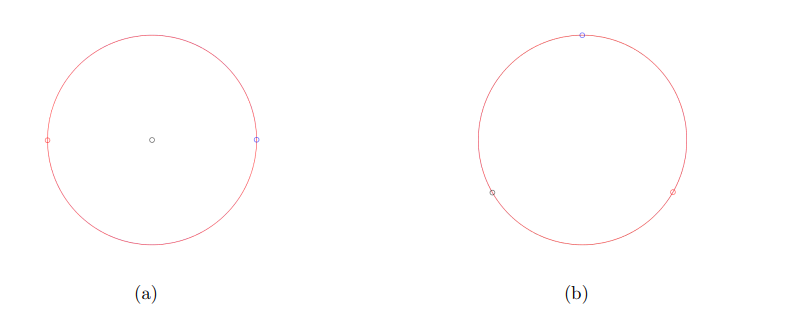
\includegraphics[width=0.4\textwidth]{EulerUndLagrange.png}
	\caption[Eintrag in Abbildungsverzeichnis von Grumpy Cat]{Klassische Drei-Körper-Orbits: (a) Euler-Orbit, (b) Lagrange-Orbit.}
	\label{EulerUndLagrange .}
\end{figure}

\paragraph{2- Figure-8: }
Der sogenannte Figure-8 Orbit ist die einzige bekannte stabile Lösung des Drei-Körper-Problems. In diesem Orbit starten die drei Körper in einer kollinearen Konfiguration und bewegen sich entlang einer 8-förmigen Bahn (Siehe Abb.3).

\begin{figure}[H]
    \centering
    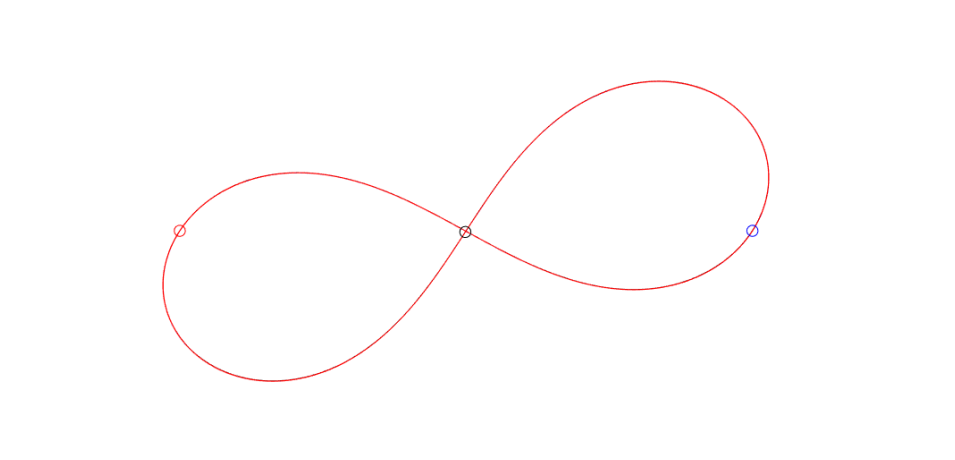
\includegraphics[width=0.6\textwidth]{figure8Orbit.png}
    \caption{Figure-8 Orbit.}
    \label{fig:figure8Orbit}
\end{figure}

Um diesen Orbit zu konstruieren, können wir die Integrale der Bewegung verwenden, 
zusammen mit der Bedingung, dass die drei Körper in einer kollinearen Konfiguration (Euler-Konfiguration) starten, um die Anzahl der zu spezifizierenden Parameter zu reduzieren. 
Wenn die Anfangspositionen in einer Euler-Konfiguration gesetzt werden, erhalten wir fünf Einschränkungen für die Positionen der Körper (sie wurden auf der x-Achse gewählt), bis hin zum Abstand der beiden äußeren Körper zum zentralen Körper, der ohne Verlust der Allgemeinheit auf 1 gesetzt werden kann (dies würde nur zu einem allgemeinen Skalierungsfaktor in der potentiellen Energie führen, und somit die Größe der Anfangsgeschwindigkeiten beeinflussen). 
Durch Arbeiten im Bezugssystem des Schwerpunkts können wir $P = 0$ setzen, was zwei Einschränkungen für die Parameter ergibt. Darüber hinaus handelt es sich um einen Orbit mit null Drehimpuls, d.h., $L = 0$, was eine weitere Einschränkung liefert. Die Erhaltung der Energie liefert die letzte Einschränkung, wodurch uns nur noch zwei ``freie" Parameter verbleiben, $v_x$ und $v_y$, die beiden Komponenten der Geschwindigkeit eines der drei Körper, wobei dieser auf der Position (1, 0) gewählt wurde. Um den Figure-8 Orbit zu erzeugen, lauten die Werte dieser Parameter:
\begin{equation}
	v_x = 0.3471128135672417, \quad v_y = 0.532726851767674
	\label{ref1}
\end{equation}


\paragraph{3- Andere Orbits: } 
Die Figur-8-Orbit-Methode ermöglicht die Identifizierung einer Vielzahl alternativer Orbits (die allesamt instabil sind), durch die Angabe unterschiedlicher Werte für $v_x$ und $v_y$.
Einige dieser anderen Orbits sind in Abbildung \ref{Abb:andereOrbits} gezeigt, mit den Werten von $v_x$ und $v_y$, die unter den Abbildungen angegeben sind.

\begin{figure}[H]
    \centering
    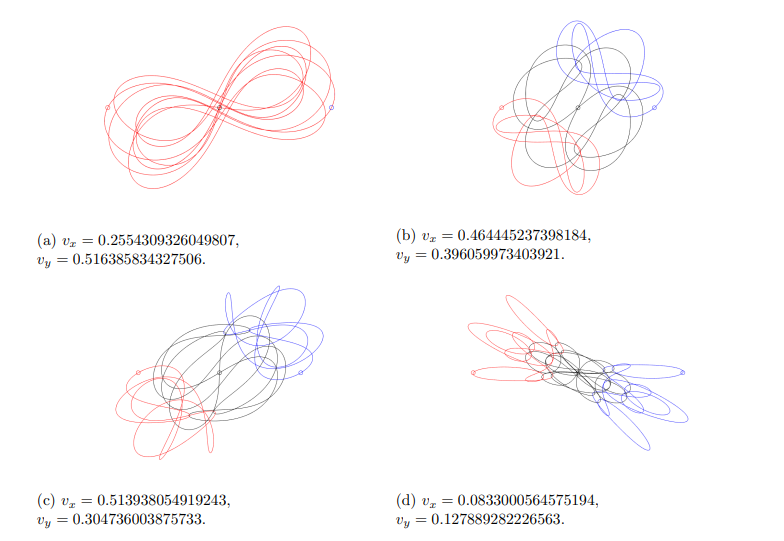
\includegraphics[width=0.6\textwidth]{AndereOrbits.png}
    \caption{Andere Orbits.}
    \label{Abb:andereOrbits}
\end{figure}

\subsubsection{Integration Methoden}
Zur Lösung des Systems von gewöhnlichen Differentialgleichungen (DGL), das die Bewegung der Körper beschreibt, ist der Einsatz eines numerischen Solvers erforderlich, um eine approximative Lösung zu erhalten. Es existiert eine Vielzahl von Solvern, die je nach ihrer Genauigkeit (Ordnung) sowie den spezifischen Eigenschaften, die sie aufweisen, ausgewählt werden können.

\paragraph{4.1 Euler-Verfahren: }
Dies ist der einfachste numerische DGL-Solver. Für ein System, das in Vektorschreibweise als $ \dot{y} = f(t, y) $, und mit einem Zeitschritt $\delta t$, geschrieben wird, wird der Wert von $y$ zum Zeitpunkt $t + \delta t$, $y_{i+1}$, in Bezug auf den Wert von $y$ zum Zeitpunkt $t$, $y_i$, berechnet als:

\begin{equation*}
    y_{i+1} = y_i + f(t, y_i)\delta t
\end{equation*}
Dies ist ein Verfahren erster Ordnung, d.h. der Fehler in der Näherung ist von der Ordnung $\delta t$. Dies macht das Verfahren sehr ungenau, und es ist notwendig, einen sehr kleinen Zeitschritt anzugeben, um eine gute Näherung zu erhalten.


\paragraph{Runge-Kutta-Verfahren vierter Ordnung}
Das Runge-Kutta-Verfahren vierter Ordnung (rk4-Verfahren) ist eine Erweiterung des Euler-Verfahrens, das die Genauigkeit verbessert, indem mehr Auswertungen des Systems pro Schritt vorgenommen werden. Für ein System, das in Vektorschreibweise als $\dot{y} = f(t, y)$ und mit einem Zeitschritt $\delta t$ geschrieben wird, wird der Wert von $y$ zum Zeitpunkt $t + \delta t$, $y_{i+1}$, in Bezug auf den Wert von $y$ zum Zeitpunkt $t$, $y_i$, berechnet als:

\begin{align*}
    k_1 &= f(t, y_i)\delta t \\
    k_2 &= f\left(t + \frac{\delta t}{2}, y_i + \frac{k_1}{2} \delta t \right) \delta t \\
    k_3 &= f\left(t + \frac{\delta t}{2}, y_i + \frac{k_2}{2} \delta t \right) \delta t \\
    k_4 &= f(t + \delta t, y_i + k_3 \delta t) \delta t \\
    y_{i+1} &= y_i + \frac{1}{6}(k_1 + 2k_2 + 2k_3 + k_4)
\end{align*}

Dies ist ein Verfahren vierter Ordnung, d.h., der Fehler in der Näherung hat die Ordnung $(\delta t)^4$. Dies macht das Verfahren deutlich genauer als das Euler-Verfahren. Zum Vergleich mit dem Euler-Verfahren müssen wir denselben Zeitschritt $\delta t$ wählen, aber viermal so viele Auswertungen pro Zeitschritt vornehmen, da das rk4-Verfahren viermal so viele Auswertungen des Systems pro Zeitschritt erfordert.




\subsection{N-Körper Problem}
Das n-Körper-Problem ist ein klassisches Problem in der Physik und beschreibt die Bewegung mehrerer Massenpunkte, die sich gegenseitig durch ihre Gravitationskräfte beeinflussen. Die Grundgleichung für die Beschleunigung eines Körpers \( j \) in einem solchen System ist gegeben durch:

\[
m_j \ddot{\mathbf{q}}_j = G \sum_{\substack{k=1 \\ k \neq j}}^n \frac{m_j m_k (\mathbf{q}_k - \mathbf{q}_j)}{|\mathbf{q}_k - \mathbf{q}_j|^3}
\]

Hier steht \( m_j \) für die Masse des betrachteten Körpers, \( \mathbf{q}_j \) für dessen Position, und \( G \) für die Gravitationskonstante. Die Summe erstreckt sich über alle anderen Körper \( k \) (mit \( k \neq j \)), die eine Gravitationskraft auf den Körper \( j \) ausüben. Der Ausdruck \( \frac{\mathbf{q}_k - \mathbf{q}_j}{|\mathbf{q}_k - \mathbf{q}_j|^3} \) beschreibt dabei die Richtung und Stärke der Gravitationskraft zwischen den beiden Körpern \( j \) und \( k \), wobei der Abstand \( |\mathbf{q}_k - \mathbf{q}_j| \) hoch drei im Nenner steht, um sicherzustellen, dass die Kraft gemäß dem Gravitationsgesetz mit dem Quadrat des Abstands abnimmt.

Das n-Körper-Problem stellt eine Herausforderung dar, weil ab mehr als zwei Körpern eine chaotische Dynamik entsteht, die eine exakte analytische Lösung unmöglich macht. Während das Zwei-Körper-Problem stabile, vorhersagbare Bahnen liefert, wird das System bei drei oder mehr Körpern extrem empfindlich gegenüber Anfangsbedingungen.
Dadurch sind die Bewegungen der Körper langfristig unvorhersehbar und schwer exakt zu berechnen. Numerische Simulationen, die die Bewegung der Körper Schritt für Schritt berechnen, bieten eine Lösungsmöglichkeit, jedoch nur in Form von Näherungen. Die Berechnungen sind dabei extrem aufwendig, da für jede Wechselwirkung die Kräfte separat berücksichtigt werden müssen, was bei steigender Körperanzahl exponentiell mehr Rechenleistung erfordert.


\section{Material und Methoden}

\subsection{Der Barnes-Hut-Algorithmus}
Der Barnes-Hut-Algorithmus ist ein effizientes Näherungsverfahren zur Berechnung der Kräfte in N-Körper-Problemen, insbesondere in der Astrophysik. Er wurde 1986 von Josh Barnes und Piet Hut entwickelt und reduziert den Rechenaufwand von $O(N^2)$ auf $O(N \log N)$, wodurch Simulationen mit einer großen Anzahl von Teilchen ermöglicht werden.
Der Algorithmus basiert auf der Annahme, dass Gruppen von weit entfernten Teilchen als einzelne Massepunkte behandelt werden können. Dazu wird der Raum rekursiv in immer kleinere Bereiche unterteilt, bis jeder Bereich entweder leer ist oder genau ein Teilchen enthält. Diese Struktur wird in Form eines Baumes, genauer eines Quadtrees im zweidimensionalen Raum oder eines Octrees im dreidimensionalen Raum, dargestellt.

\subsubsection{Algorithmusschritte}

\paragraph{1. Baumerstellung}
Der gesamte Raum wird in vier (2D) bzw. acht (3D) Quadranten unterteilt. Jedes Teilchen wird entsprechend seiner Position in einen dieser Quadranten einsortiert. Ist ein Quadrant bereits belegt, wird er weiter unterteilt, bis jedes Teilchen in einem eigenen Unterquadranten liegt. Dieses rekursive Unterteilen führt zur Bildung des Quadtrees bzw. Octrees.

\paragraph{2. Masseverteilung}
Nach der Baumerstellung wird für jeden Knoten des Baumes die Gesamtmasse und der Massenschwerpunkt der in ihm enthaltenen Teilchen berechnet. Diese Informationen sind entscheidend für die spätere Kraftberechnung.

\paragraph{3. Kraftberechnung}
Um die auf ein bestimmtes Teilchen wirkende Kraft zu berechnen, wird der Baum erneut durchlaufen. Für jeden Knoten wird das Verhältnis von dessen Größe zur Entfernung zum betrachteten Teilchen berechnet. Ist dieses Verhältnis kleiner als ein vorgegebener Schwellenwert ($\theta$), wird der gesamte Knoten als eine einzelne Masse im Massenschwerpunkt betrachtet. Andernfalls werden die Unterknoten weiter untersucht. Dieses Verfahren reduziert die Anzahl der notwendigen Kraftberechnungen erheblich.

\subsubsection{Parameter $\theta$}
Der Schwellenwert $\theta$ bestimmt die Genauigkeit der Näherung. Ein kleiner Wert für $\theta$ führt zu einer höheren Genauigkeit, da weniger Gruppierungen vorgenommen werden und mehr direkte Berechnungen stattfinden. Ein größerer Wert reduziert den Rechenaufwand, kann jedoch die Genauigkeit beeinträchtigen. Typischerweise wird $\theta$ auf Werte um 0,5 bis 1 gesetzt, abhängig von den Anforderungen an die Simulation.

\subsubsection{Vorteile und Anwendungen}
Der Barnes-Hut-Algorithmus ermöglicht die Simulation von Systemen mit Millionen von Teilchen, was mit direkten Berechnungsmethoden unpraktikabel wäre. Er findet Anwendung in der Astrophysik, beispielsweise bei der Simulation von Galaxien, sowie in anderen Bereichen wie der Molekulardynamik und der Informatik, etwa beim kräftebasierten Zeichnen von Graphen.

\subsection{React.js -- Funktionsweise und Anwendungen}

React.js ist eine JavaScript-Bibliothek, die zur Entwicklung von Benutzeroberflächen verwendet wird. Sie basiert auf einer komponentenbasierten Architektur, bei der Anwendungen in wiederverwendbare, eigenständige Komponenten unterteilt werden. Jede Komponente verwaltet ihre eigenen Daten und ihr Verhalten. Dies erleichtert die Pflege und Erweiterung komplexer Anwendungen. Ein zentrales Merkmal von React.js ist das virtuelle DOM. Statt Änderungen direkt im echten DOM vorzunehmen, werden diese zunächst im virtuellen DOM simuliert. Anschließend werden nur die tatsächlich geänderten Elemente in den echten DOM übernommen. Dieser Ansatz verbessert die Leistung erheblich, insbesondere bei Anwendungen mit häufigen Aktualisierungen.

Ein weiteres wichtiges Konzept in React.js ist der unidirektionale Datenfluss. Daten werden von Eltern- zu Kinderkomponenten weitergegeben, was die Vorhersagbarkeit und Wartbarkeit des Codes erhöht. Seit der Einführung von React Hooks in Version 16.8 können Entwickler Zustände und Lebenszyklusmethoden in funktionalen Komponenten verwenden. Hooks wie \texttt{useState} und \texttt{useEffect} vereinfachen die Verwaltung von Zuständen und Nebenwirkungen.

\subsubsection{Anwendungen von React.js}
React.js eignet sich besonders gut für Single-Page Applications (SPAs). In solchen Anwendungen werden nur die benötigten Inhalte aktualisiert, anstatt komplette Seiten neu zu laden. Dies führt zu einer flüssigen und reaktionsschnellen Benutzererfahrung. Darüber hinaus ist React.js ideal für datenintensive Anwendungen, wie z.B. Dashboards und Simulationen, die häufige Aktualisierungen und eine effiziente Verwaltung des Zustands erfordern. Weitere Anwendungen finden sich in der Datenvisualisierung, insbesondere in Kombination mit Bibliotheken wie D3.js und Chart.js, sowie in interaktiven Simulationen und Modellen.

\subsubsection{Warum eignet sich React.js für den Barnes-Hut-Algorithmus?}
React.js bietet eine ideale Grundlage für die Implementierung des Barnes-Hut-Algorithmus, da dieser auf häufigen Aktualisierungen und dynamischen Daten basiert. Das virtuelle DOM sorgt dafür, dass nur die tatsächlich betroffenen Teile der Benutzeroberfläche aktualisiert werden. Dies ist besonders wichtig bei der Visualisierung von Simulationen mit vielen Teilchen, bei denen laufend neue Positionen und Kräfte berechnet werden.

Die komponentenbasierte Struktur von React.js ermöglicht es, jede Simulationseinheit -- sei es ein Teilchen oder ein Knoten im Baum -- als eigenständige Komponente zu modellieren. Dies erleichtert die Verwaltung von Zuständen und Interaktionen innerhalb der Simulation. Mit React Hooks wie \texttt{useState} und \texttt{useEffect} können diese Zustände effizient aktualisiert werden, ohne den gesamten Baum neu zu rendern.

Ein weiterer Vorteil ist die einfache Integration von Bibliotheken zur Datenvisualisierung und physikalischen Modellierung. Bibliotheken wie D3.js oder Three.js können nahtlos in React-Projekte eingebunden werden, um komplexe Darstellungen und Animationen zu erzeugen. Darüber hinaus unterstützt React.js den Einsatz von WebGL, was eine hardwarebeschleunigte Darstellung von Simulationen ermöglicht.

Zusammenfassend bietet React.js durch seine Effizienz, Modularität und Erweiterbarkeit eine ideale Plattform zur Implementierung von Simulationen auf Basis des Barnes-Hut-Algorithmus. Dies macht es zu einer bevorzugten Wahl für Anwendungen, die sowohl hohe Leistung als auch eine interaktive Benutzeroberfläche erfordern.

\subsection{Vorgehensweise und Implementierung}

\section{Resultat}
\subsection{Vergleich der Simulationsergebnisse}

\section{Diskussion}
\subsection{Vorteile der verwendeten Algorithmen}
\subsection{Herausforderungen und Limitierungen}
\subsection{Vergleich mit bestehenden Methoden}

\section{Schlussfolgerung}
\section{Literaturverzeichnis}
\section{Abbildungsverzeichnis}

\end{document}

